\documentclass{beamer}
\usepackage[english,russian]{babel}
\usepackage[utf8]{inputenc}
\usepackage{graphicx}
\usepackage{amssymb,amsmath}
\usepackage{float}
\usepackage{array}
\usepackage{ragged2e}
\usetheme[numbers]{Berlin}

\setbeamertemplate{caption}[numbered]
\pagestyle{plain} 
\setcounter{page}{0}


\begin{document}

\institute{МГУ имени М.В. Ломоносова, Москва, Россия}
\title{Отчет о выполнении II задания практикума}  
\author{Григорьева О. Константинова М. Козодой А.}
\date{ 2017\\Москва} 
\thispagestyle{empty}
\frame{\titlepage} 

\begin{frame}{Описание задания}
	После оглушительного успеха в освобождении Астапора, Миэрина и Юнкая от власти работорговцев Дейенерис Бурерожденная открыла себе доступ к Летнему морю, а следовательно -- путь в Вестерос.
	Для ведения войны с Семью Королевствами нужно оружие, а для оружия нужна сталь. Нет никаких сомнений в кузнечном искусстве Безупречных, однако поставщики стали не столь надежны.
	Два основных поставщика стали -- это Westeros Inc. и Harpy & Co. 
\end{frame}

\begin{frame}{Описание задания}
	На протяжении нескольких месяцев мы закупаем сталь у обеих компаний, и каждая из них предлагает ощутимую скидку при заключении эксклюзивного договора на поставку.
	Советник королевы Тирион Ланнистер знает о твоем умении принимать взвешенные рациональные решения и просит помощи в объективном решении вопроса о том, с какой из компаний следует заключить эксклюзивный договор на поставку стали.
	У Тириона есть записи о производстве мечей каждым из кузнецов-безупречных, а также данные о количестве сломанных мечей в каждый из месяцев ведения боевых действий.
\end{frame}


\begin{frame}{Выполнение задания}
Необходимо провести разведывательный анализ данных с целью ответа на вопрос: "С каким из поставщиков стали следует заключить договор?" Работа ведется с  данными за прошедшие 7 месяцев из CSV-файла.	
Для этого считываем CSV-файл в матрицу и описываем необходимые нам для работы переменные.
Далее разделяем поток данных по двум компаниям, а для этого считаем два вектора prod{\_}sum{\_}co и prod{\_}sum{\_}inc соответсвующие двум компаниям - Harpy&co и Westeros incorporate соовественно.
Каждый вектор содержит 6 значений, которые вычисляются по принципу:
1 месяц : производство за 1 месяц минус суммарный брак за 6 месяцев, и суммируется все по 50 кузнецам
2 месяц, соответственно, производство 2-ого минус суммарный брак, наблюдаемый за 5 месяцев и так далее.
\end{frame}

\begin{frame}{Выполнение задания}
Диаграммы размахов, или "ящики с усами" (англ. box-whisker plots), получили свое название за характерный вид: точку или линию, соответствующую медианe, окружает прямоугольник ("ящик"), длина которого соответствует одному из показателей разброса или точности оценки генерального параметра. Дополнительно от этого прямоугольника отходят "усы", также соответствующие по длине одному из показателей разброса или точности. Графики этого типа очень популярны, поскольку позволяют дать очень полную статистическую характеристику анализируемой совокупности. Кроме того, диаграммы размаха можно использовать для визуальной экспресс-оценки разницы между двумя и более группами
\end{frame}

\begin{frame}{Выполнение задания}
Далее строим описанный выше "ящики с усами"  для обеих компаний-производителей по таблице в которой первый столбец - это значения векторов, второй столбец соответсвующее название компании. 
Для этого используем функцию boxplot() и обозначаем диаграмму Harpy.co красным цветом, а Westeros.Inc - желтым.

\end{frame}

\begin{frame}{Выполнение задания}	
	\begin{figure}[h]
		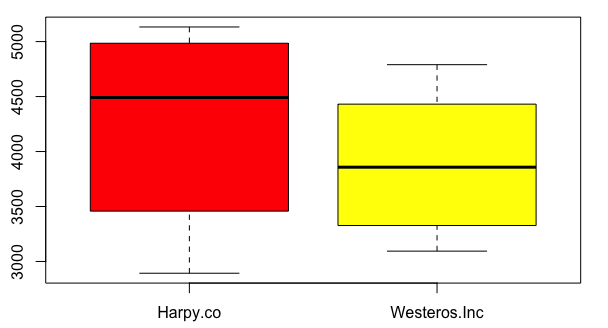
\includegraphics[width=100mm]{ysi}
		\caption{"Ящики с усами"}
		\label{ysi}
	\end{figure}
\end{frame}

\begin{frame}{Анализ результатов}
Как видно на рисунке, медиана Harpy.co выше медианы Westeros.Inc, пусть и разброс у первой компании больше. Высота медианы показывает, что показатели Harpy.co выше, а следовательно советнику Бурерожденной Тириону стоит посоветовать своей госпоже именно эту компанию.
\end{frame}

\begin{frame}{Задание выполняли}
	\begin{itemize}
		{\tiny \item Григорьева Олеся, студентка 412 группы. Занималась разработкой подхода и написанием программы.
		\item Константинова Мария, студентка 412 группы. Разрабатывала подход к решению и писала отчет.
		\item Козодой Антон, студент 412 группы. Писал отчет и проводил анализ результатов.
				}
	\end{itemize}	
	\begin{figure}[h]
		
\includegraphics[width=50mm]{tron}
		\caption{"Он будет нашим"}
		\label{tron}
	\end{figure}

\end{frame}

\end{document}
